	\documentclass{article}
\usepackage[utf8]{inputenc}
\usepackage{graphicx}
\usepackage{amsmath}
\usepackage{titling}
\usepackage{pdflscape}
\usepackage[export]{adjustbox}
\usepackage{float}

\setlength{\droptitle}{-10em}
\pagestyle{empty}

\title{Lab. 2 - La rete dei trasporti pubblici}
\author{Ballarin Simone, Gobbo Alessio, Rossi Daniel}
\date{April 2019}

\begin{document}
\maketitle

\section*{Domanda 1}
La rete di traporti è stata modellata come segue:
\begin{itemize}
	\item \textbf{Vertici}: stazioni
	\item \textbf{Archi}: trasporti tra una stazione ed un'altra.
\end{itemize}
Ogni arco da una stazione A ad una stazione B tiene come peso l'orario di partenza da A e di arrivo a B.
Più nel dettaglio abbiamo deciso di utilizzare come lista delle adianceze per ciascun nodo un dizionario, avente per chiave la stazione di arrivo e per valore una lista ordinata per orario di partenza delle corse con partenza dalla stazione corrente a quella chiave.

\section*{Domanda 2}
Abbiamo implementato sia l'algoritmo Dijkstra sia l'algoritmo A*, utilizzando per entrambi un min-heap come coda di priorità, rispetto l'algoritmo visto a lezione si è deciso di inglobare la funzione di inizializzazione e la funzione di rilassamento all'interno della struttura dati min-heap.

\section*{Domanda 3}

\begin{figure}[H]
	\begin{minipage}{0.55\linewidth}
		\centering
		\hspace*{-6cm}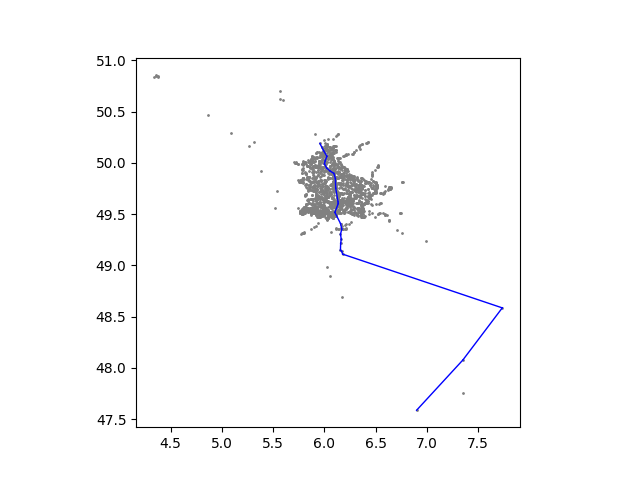
\includegraphics[width=1.0\linewidth, valign=t]{figures/Figure_1}
	\end{minipage}
	\hspace*{-4cm}\begin{minipage}{0.7\linewidth}
		\textbf{Viaggio 1}:\\
		Viaggio da 200415016 a 200405005\\
		Orario di partenza: 09:30\\
		Orario di arrivo: 09:52\\
		09:30 corsa 00360 RGTR125/1 da 200415016 a 200415009\\
		09:50 corsa 06602 RGTR10 da 200415009 a 200405005
			\end{minipage}
\end{figure}
\begin{figure}[H]
	\begin{minipage}{0.55\linewidth}
		\centering
		\hspace*{-6cm}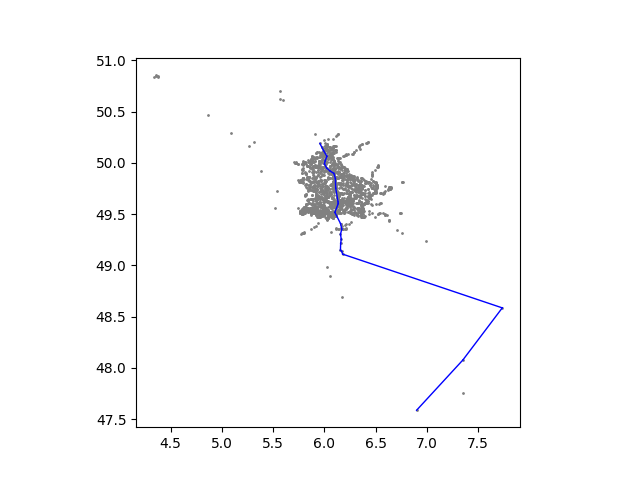
\includegraphics[width=1.0\linewidth, valign=t]{figures/Figure_1}
	\end{minipage}
	\hspace*{-4cm}\begin{minipage}{0.7\linewidth}
		\textbf{Viaggio 2}:\\
		Viaggio da 300000032 a 400000122\\
		Orario di partenza: 05:30\\
		Orario di arrivo: 13:50\\
		06:26 corsa 07608 C881 da 300000032 a 110606001\\
		07:26 corsa 03781 C821 da 110606001 a 200417051\\
		07:46 corsa 00055 C82TER da 200417051 a 220102005\\
		12:07 corsa 09879 C821 da 220102005 a 400000122
		
			\end{minipage}
\end{figure}
\begin{figure}[H]
	\begin{minipage}{0.55\linewidth}
		\centering
		\hspace*{-6cm}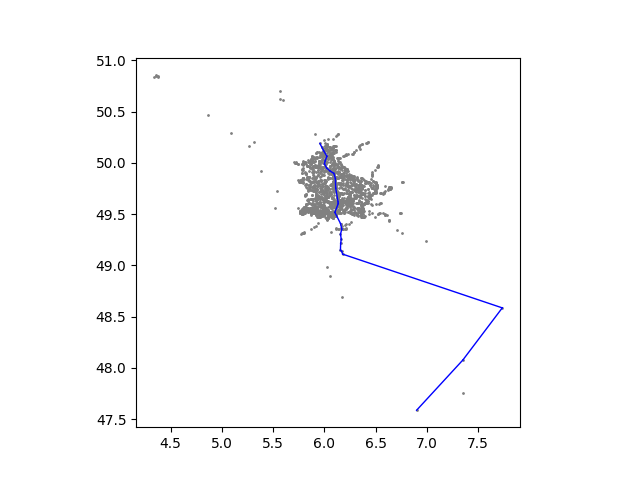
\includegraphics[width=1.0\linewidth, valign=t]{figures/Figure_1}
	\end{minipage}
	\hspace*{-4cm}\begin{minipage}{0.7\linewidth}
		\textbf{Viaggio 3}:\\
		Viaggio da 210602003 a 300000030\\
		Orario di partenza: 06:30\\
		Orario di arrivo: 10:53\\
		06:41 corsa 00030 CFLBUS185 da 210602003 a 210602005\\
		06:55 corsa 00037 CFLBUS175 da 210602005 a 220502003\\
		07:07 corsa 01306 CFLBUS176 da 220502003 a 201103001\\
		07:20 corsa 00024 RGTR176 da 201103001 a 200405036\\
		07:24 corsa 01173 RGTR172 da 200405036 a 200405026\\
		07:27 corsa 04301 AVL31 da 200405026 a 200405035\\
		07:40 corsa 07630 C821 da 200405035 a 300000030
			\end{minipage}
\end{figure}
\begin{figure}[H]
	\begin{minipage}{0.55\linewidth}
		\centering
		\hspace*{-6cm}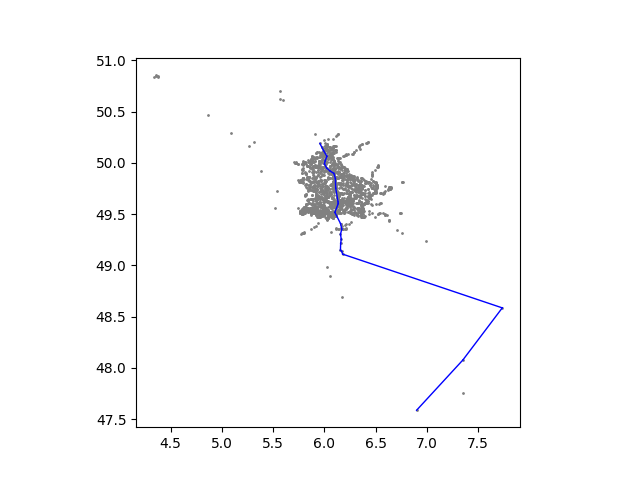
\includegraphics[width=1.0\linewidth, valign=t]{figures/Figure_1}
	\end{minipage}
	\hspace*{-4cm}\begin{minipage}{0.7\linewidth}
		\textbf{Viaggio 4}:\\
		Viaggio da 200417051 a 140701016\\
		Orario di partenza: 12:00\\
		Orario di arrivo: 12:43\\
		12:20 corsa 03712 C821 da 200417051 a 140701016
		
			\end{minipage}
\end{figure}
\begin{figure}[H]
	\begin{minipage}{0.55\linewidth}
		\centering
		\hspace*{-6cm}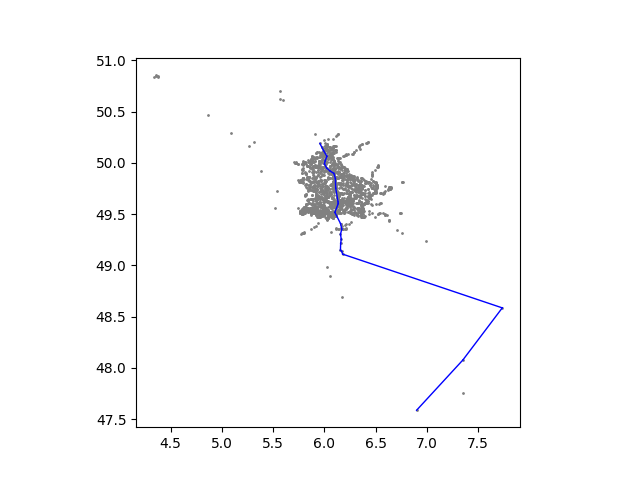
\includegraphics[width=1.0\linewidth, valign=t]{figures/Figure_1}
	\end{minipage}
	\hspace*{-4cm}\begin{minipage}{0.7\linewidth}
		\textbf{Viaggio 5}:\\
		Viaggio da 200417051 a 140701016\\
		Orario di partenza: 23:55\\
		Orario di arrivo: 00:44\\
		00:09 corsa 03623 C821 da 200417051 a 140701016
		
	\end{minipage}
\end{figure}
\begin{figure}[H]
	\begin{minipage}{0.55\linewidth}
		\centering
		\hspace*{-6cm}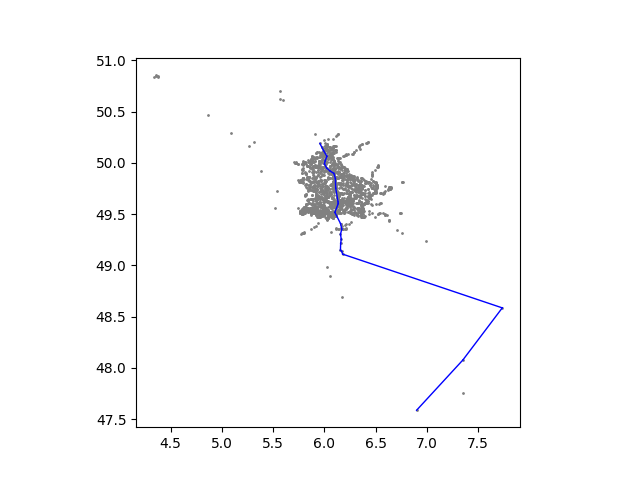
\includegraphics[width=1.0\linewidth, valign=t]{figures/Figure_1}
	\end{minipage}
	\hspace*{-4cm}\begin{minipage}{0.7\linewidth}
		\textbf{Viaggio 6}:\\
		Viaggio da 200406015 a 110405001\\
		Orario di partenza: 21:30\\
		Orario di arrivo: 07:16\\
		21:45 corsa 02708 AVL20 da 200406015 a 200406013\\
		21:47 corsa 03714 AVLCN da 200406013 a 200406011\\
		21:57 corsa 00487 RGTR125/1 da 200406011 a 200405020\\
		22:03 corsa 03714 AVLCN da 200405020 a 200405023\\
		22:12 corsa 03725 AVLCN da 200405023 a 200405035\\
		22:16 corsa 03722 C821 da 200405035 a 200417051\\
		04:30 corsa 03468 RGTR840 da 200417051 a 110101004\\
		07:14 corsa 02156 RGTR665 da 110101004 a 110405001
		
			\end{minipage}
\end{figure}
\begin{figure}[H]
	\begin{minipage}{0.55\linewidth}
		\centering
		\hspace*{-6cm}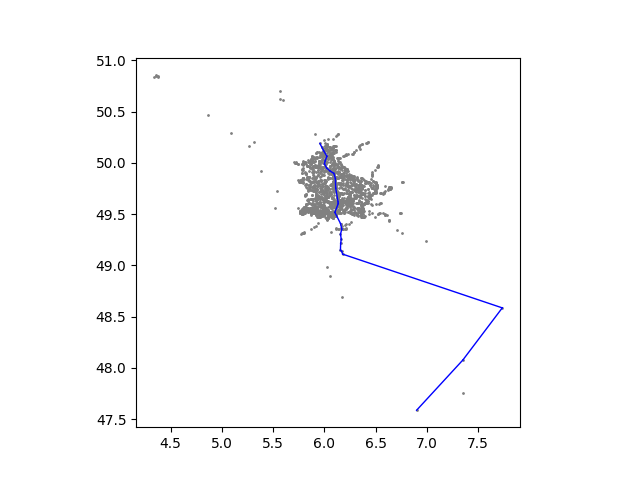
\includegraphics[width=1.0\linewidth, valign=t]{figures/Figure_1}
	\end{minipage}
	\hspace*{-4cm}\begin{minipage}{0.7\linewidth}
		\textbf{Viaggio 7}:\\
		Viaggio da 140701040 a 210101001\\
		Orario di partenza: 05:30\\
		Orario di arrivo: 07:10\\
		05:34 corsa 06082 RGTR512 da 140701040 a 140701013\\
		05:45 corsa 03830 C821 da 140701013 a 160904001\\
		06:12 corsa 03626 CFLBUSL10 da 160904001 a 200419026\\
		06:20 corsa 03177 AVL4 da 200419026 a 200405014\\
		06:22 corsa 00040 AVL18 da 200405014 a 200417047\\
		06:34 corsa 05313 RGTR213 da 200417047 a 200417044\\
		06:41 corsa 00693 RGTR194 da 200417044 a 200601006\\
		06:51 corsa 02907 RGTR160 da 200601006 a 210101001
		
			\end{minipage}
\end{figure}
\begin{figure}[H]
	\begin{minipage}{0.55\linewidth}
		\centering
		\hspace*{-6cm}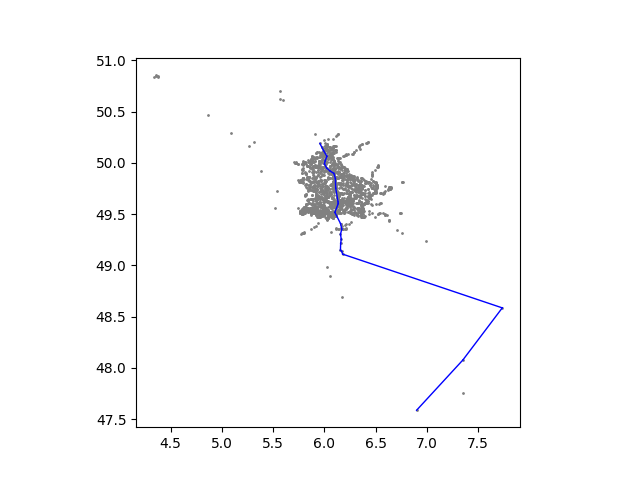
\includegraphics[width=1.0\linewidth, valign=t]{figures/Figure_1}
	\end{minipage}
	\hspace*{-4cm}\begin{minipage}{0.7\linewidth}
		\textbf{Viaggio 8}:\\
		Viaggio da 170801001 a 220402082\\
		Orario di partenza: 12:30\\
		Orario di arrivo: 14:44\\
		12:45 corsa 03018 RGTR414 da 170801001 a 160501003\\
		12:59 corsa 01007 RGTR100 da 160501003 a 160601001\\
		13:07 corsa 01473 RGTR409 da 160601001 a 160601008\\
		13:26 corsa 03737 C821 da 160601008 a 200417051\\
		13:44 corsa 08000 RGTR27 da 200417051 a 200415003\\
		13:46 corsa 07810 RGTR200 da 200415003 a 200415002\\
		13:58 corsa 05168 RGTR205 da 200415002 a 220701003\\
		14:11 corsa 07234 RGTR321 da 220701003 a 220402106\\
		14:42 corsa 00056 TIC12 da 220402106 a 220402082
		
			\end{minipage}
\end{figure}
\end{document}
